\section{Results}

\subsection{Descriptive Statistics}

Environmental conditions varied substantially across the 78-day monitoring period at Spring Canyon and UDMH during the 2023-2024 overwintering season. The dataset comprised 1,894 observations collected at 30-minute intervals during daylight hours (07:00--17:00) from November 17, 2023, to February 4, 2024, totaling 947 observation hours across 115 unique deployment-day combinations.

Wind speeds ranged from complete calm to moderately strong conditions, with maximum gusts reaching 12.4 m/s (mean = 2.2 ± 1.4 m/s, median = 2.2 m/s). The interquartile range of 1.3--3.0 m/s indicated that most observations occurred under relatively mild wind conditions. Temperature showed considerable variation throughout the monitoring period, ranging from 3.0 to 30.0°C (mean = 14.6 ± 3.8°C, median = 14.0°C), with an interquartile range of 12.5--17.0°C typical of California coastal winter conditions. Direct solar exposure occurred in 31.7\% of observations (n = 601), with butterflies actively basking when present in sunlight, averaging 17.0 individuals in direct sun (range: 1--295).

Monarch abundance exhibited high variability across sites and time periods. Butterfly counts ranged from 0 to 770 individuals per observation, with a mean of 81.4 ± 100.0 butterflies and a median of 37 butterflies. The wide interquartile range (9--119 butterflies) reflected substantial variation in cluster sizes. Zero-count observations, representing either the beginning of cluster formation or cluster dissolution, comprised 2.3\% of the dataset (n = 43).

Cluster sizes varied markedly among the 10 deployment locations. Site SC10 recorded the largest aggregation with 770 monarchs, while mean abundances ranged from 0 at SC9 to 325.8 at UDMH2. Eight deployments observed maximum cluster sizes exceeding 100 butterflies, with mean maximum cluster size across sites reaching 315.6 individuals. This variation in cluster sizes across deployments reflects the heterogeneous distribution of monarchs across overwintering microhabitats within the study sites.

The comprehensive temporal coverage, with observations at 30-minute intervals capturing 16.5 observations per deployment-day on average, provided fine-scale resolution of monarch behavioral responses to changing environmental conditions. Peak observation activity occurred at 16:00 hours (196 observations), corresponding with afternoon warming periods when monarchs typically exhibit increased movement.

\subsection{Summary of Data and Model Selection}

Environmental factors, but not wind, drove monarch abundance changes in 1,894 paired observations from 115 monitoring periods at two overwintering sites during the 2023-2024 season. Testing of 48 candidate models identified M23 as the best-fit model.

Model M23 included smooth terms for previous butterfly count, temperature, butterflies in direct sun, and time since sunrise, achieving an AIC value of 8081.848 (Table~\ref{tab:model_selection}). This model accounted for 88\% of the model weight (AIC weight = 0.88), with the next-best model (M22) showing substantially less support (ΔAIC = 4.796). Wind variables appeared in only one of the top five models (M24), which included maximum wind speed but performed substantially worse than M23 (ΔAIC = 6.2, AIC weight = 0.04), with the wind effect showing weak evidence of an association (p = 0.218).

\begin{table}[htbp]
\centering
\caption{Model selection results showing the top five candidate models ranked by AIC. Model terms are shown with their respective AIC values, ΔAIC relative to the best model, and AIC weights across the five top performing models. Given that no models are regarded as equivalent to the best fit model (M23), the actual weight of M23 is 1.0. Wind p-values are shown where applicable; NA indicates the model did not include wind variables.}
\label{tab:model_selection}
\begin{tabular}{lllrrr}
\hline
Model & Terms & AIC & ΔAIC & Weight & Wind p \\
\hline
M23 & Previous butterfly count, Temperature, & 8081.8 & 0.0 & 0.880 & NA \\
    & Butterflies in direct sun, Time since sunrise & & & & \\
M22 & Previous butterfly count, Temperature (linear), & 8086.6 & 4.8 & 0.080 & NA \\
    & Butterflies in direct sun, Time since sunrise & & & & \\
M24 & Previous butterfly count, Maximum wind speed, & 8088.0 & 6.2 & 0.040 & 0.218 \\
    & Temperature, Butterflies in direct sun, Time since sunrise & & & & \\
M47 & Temperature, Butterflies in direct sun, & 8101.3 & 19.4 & <0.001 & NA \\
    & Time since sunrise & & & & \\
M17 & Previous butterfly count, Temperature, & 8105.9 & 24.0 & <0.001 & NA \\
    & Butterflies in direct sun & & & & \\
\hline
\end{tabular}
\end{table}

\subsection{Analysis of the Best-Fit Model}

The best-fit model (M23) explained 5.7\% of variance in monarch abundance changes (adjusted R² = 0.057). The model formula was:

\begin{equation}
\text{Change in abundance} \sim s(\text{Previous butterfly count}) + s(\text{Temperature}) + s(\text{Butterflies in direct sun}) + s(\text{Time since sunrise})
\end{equation}

where $s()$ denotes smooth terms. All four smooth terms showed significant effects on monarch abundance changes.

\begin{table}[htbp]
\centering
\caption{Summary of smooth terms in the best-fit model (M23). EDF represents effective degrees of freedom, indicating the complexity of each smooth relationship.}\label{tab:smooth_terms}
\begin{tabular}{lrrrr}
\hline
Term & EDF & Ref.~df & F-value & p-value \\
\hline
Previous butterfly count & 2.62 & 2.62 & 12.02 & 8.26e-07 \\
Temperature & 3.93 & 3.93 & 3.23 & 0.028 \\
Butterflies in direct sun & 1.53 & 1.53 & 19.36 & 1.22e-05 \\
Time since sunrise & 4.90 & 4.90 & 8.90 & <2e-16 \\
\hline
\end{tabular}
\end{table}

All four predictors in the best-fit model showed significant effects on monarch abundance changes (Figure~\ref{fig:partial_effects}). The previous butterfly count exhibited a significant non-linear negative relationship (EDF = 2.62, F = 12.02, p < 0.001), with increasingly negative changes as the previous count increased, indicating proportionally greater departures from larger aggregations. Butterflies in direct sun showed a strong negative effect on roost abundance (EDF = 1.53, F = 19.36, p < 0.001), with greater numbers in direct sun associated with larger decreases in total abundance.

Time since sunrise revealed a pronounced diurnal pattern (EDF = 4.90, F = 8.90, p < 0.001), capturing cyclical changes in monarch activity throughout the day. Temperature exhibited a complex non-linear relationship (EDF = 3.93, F = 3.23, p = 0.028), with effects peaking at approximately 20°C.

\begin{figure}[htbp]
\centering
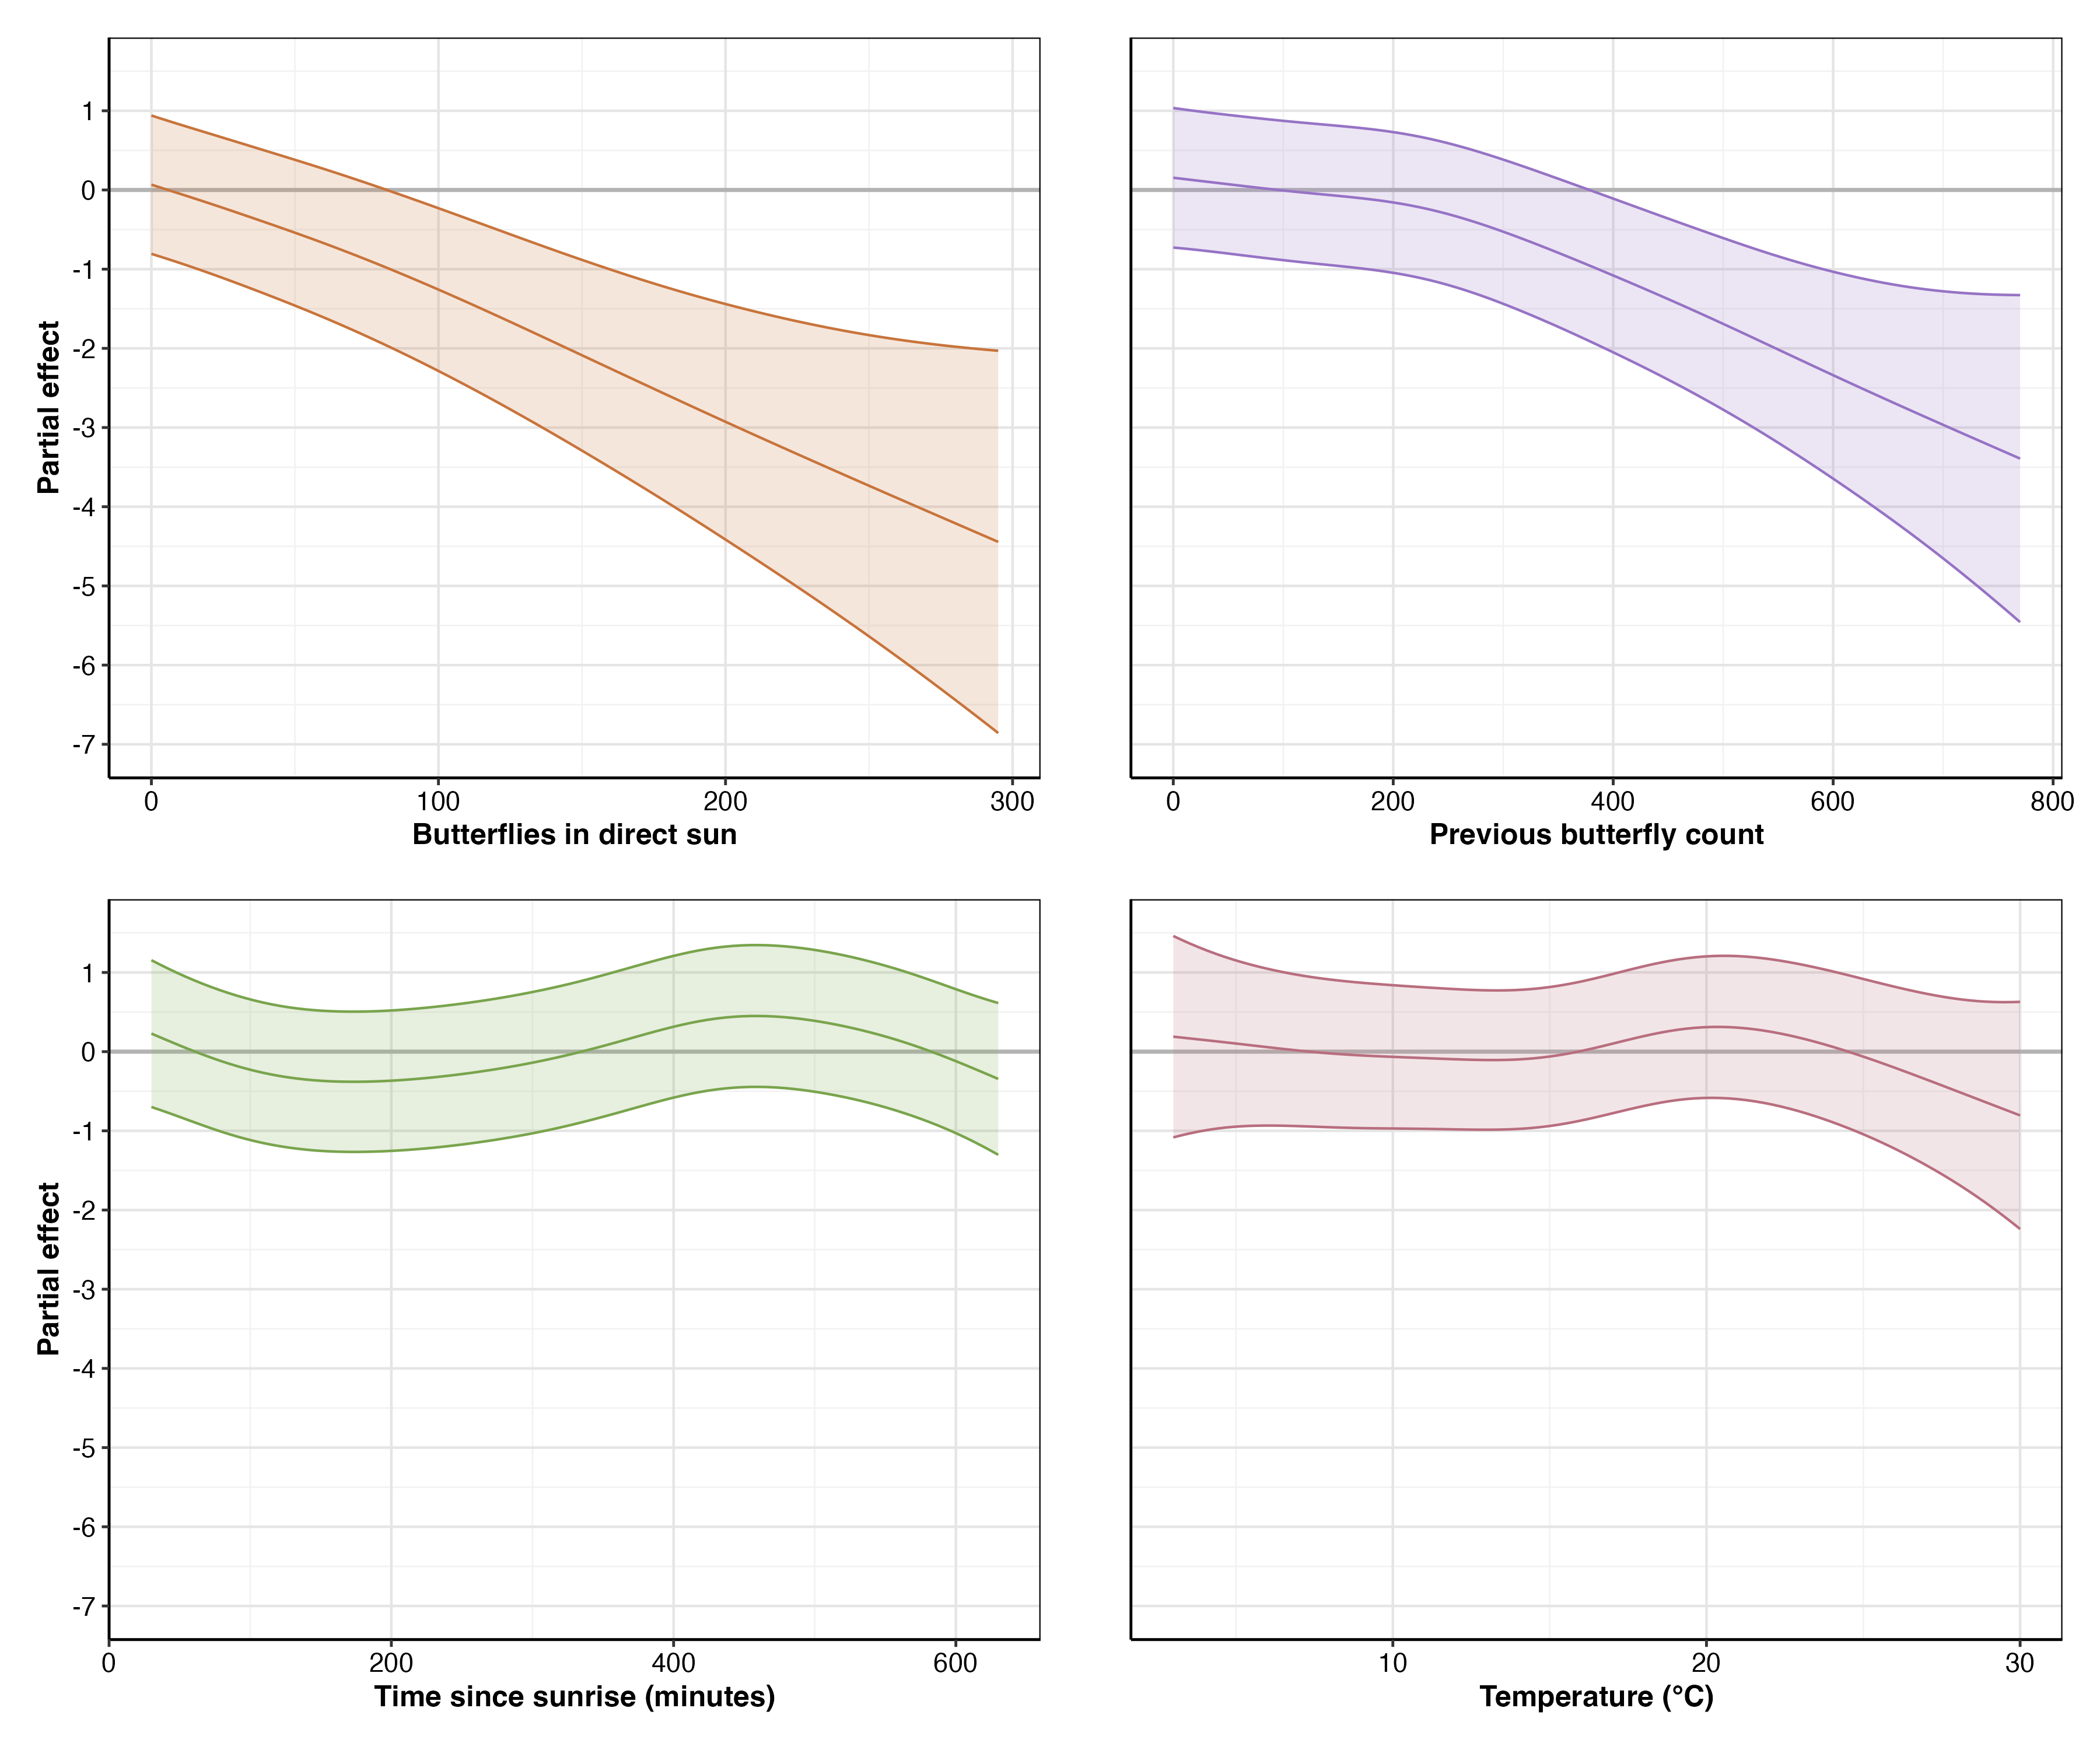
\includegraphics[width=\textwidth]{figures/results/combined_partial_effects_2x2_final.png}
\caption{Partial effects of the four significant predictors on monarch abundance change in a 2x2 layout. The partial effect on monarch abundance as estimated from the single attribute being compared to abundance while assuming all other attribute values are held constant. Top row: butterflies in direct sun (left) and previous butterfly count (right). Bottom row: time since sunrise in minutes (left) and temperature in °C (right). Solid lines show the estimated smooth functions with 95\% confidence intervals (shaded regions). All effects are shown on the same scale for comparison.}\label{fig:partial_effects}
\end{figure}

\subsection{Evaluation of the Disruptive Wind Hypothesis}

Our analysis provided no support for the three hierarchical wind hypotheses:

First, wind did not act as a disruptive force to overwintering monarchs. Among our 48 candidate models, wind appeared in only one of the top five models (M24), where it showed little evidence of an effect (p = 0.218) and resulted in substantially poorer model performance compared to the best model (ΔAIC = 6.2).

Second, we found no evidence for disruption above the proposed 2~m/s threshold. A sensitivity analysis using a specific threshold predictor ('minutes with wind speed > 2~m/s') confirmed this lack of a threshold effect, as models with this variable performed poorly and did not rank among the top candidates. Visually, the relationship between wind and monarch abundance change remained flat across the 2~m/s boundary (Figure~\ref{fig:wind_scatter}). With mean maximum wind speeds of 2.2~m/s (SD = 1.4~m/s), conditions that should have revealed threshold effects if present, no disruption occurred at or above this boundary.

Third, wind's effects did not scale with intensity. The relationship remained flat across all observed wind speeds (0–12~m/s), with confidence intervals consistently encompassing zero (Figure~\ref{fig:wind_scatter}).

\begin{figure}[htbp]
\centering
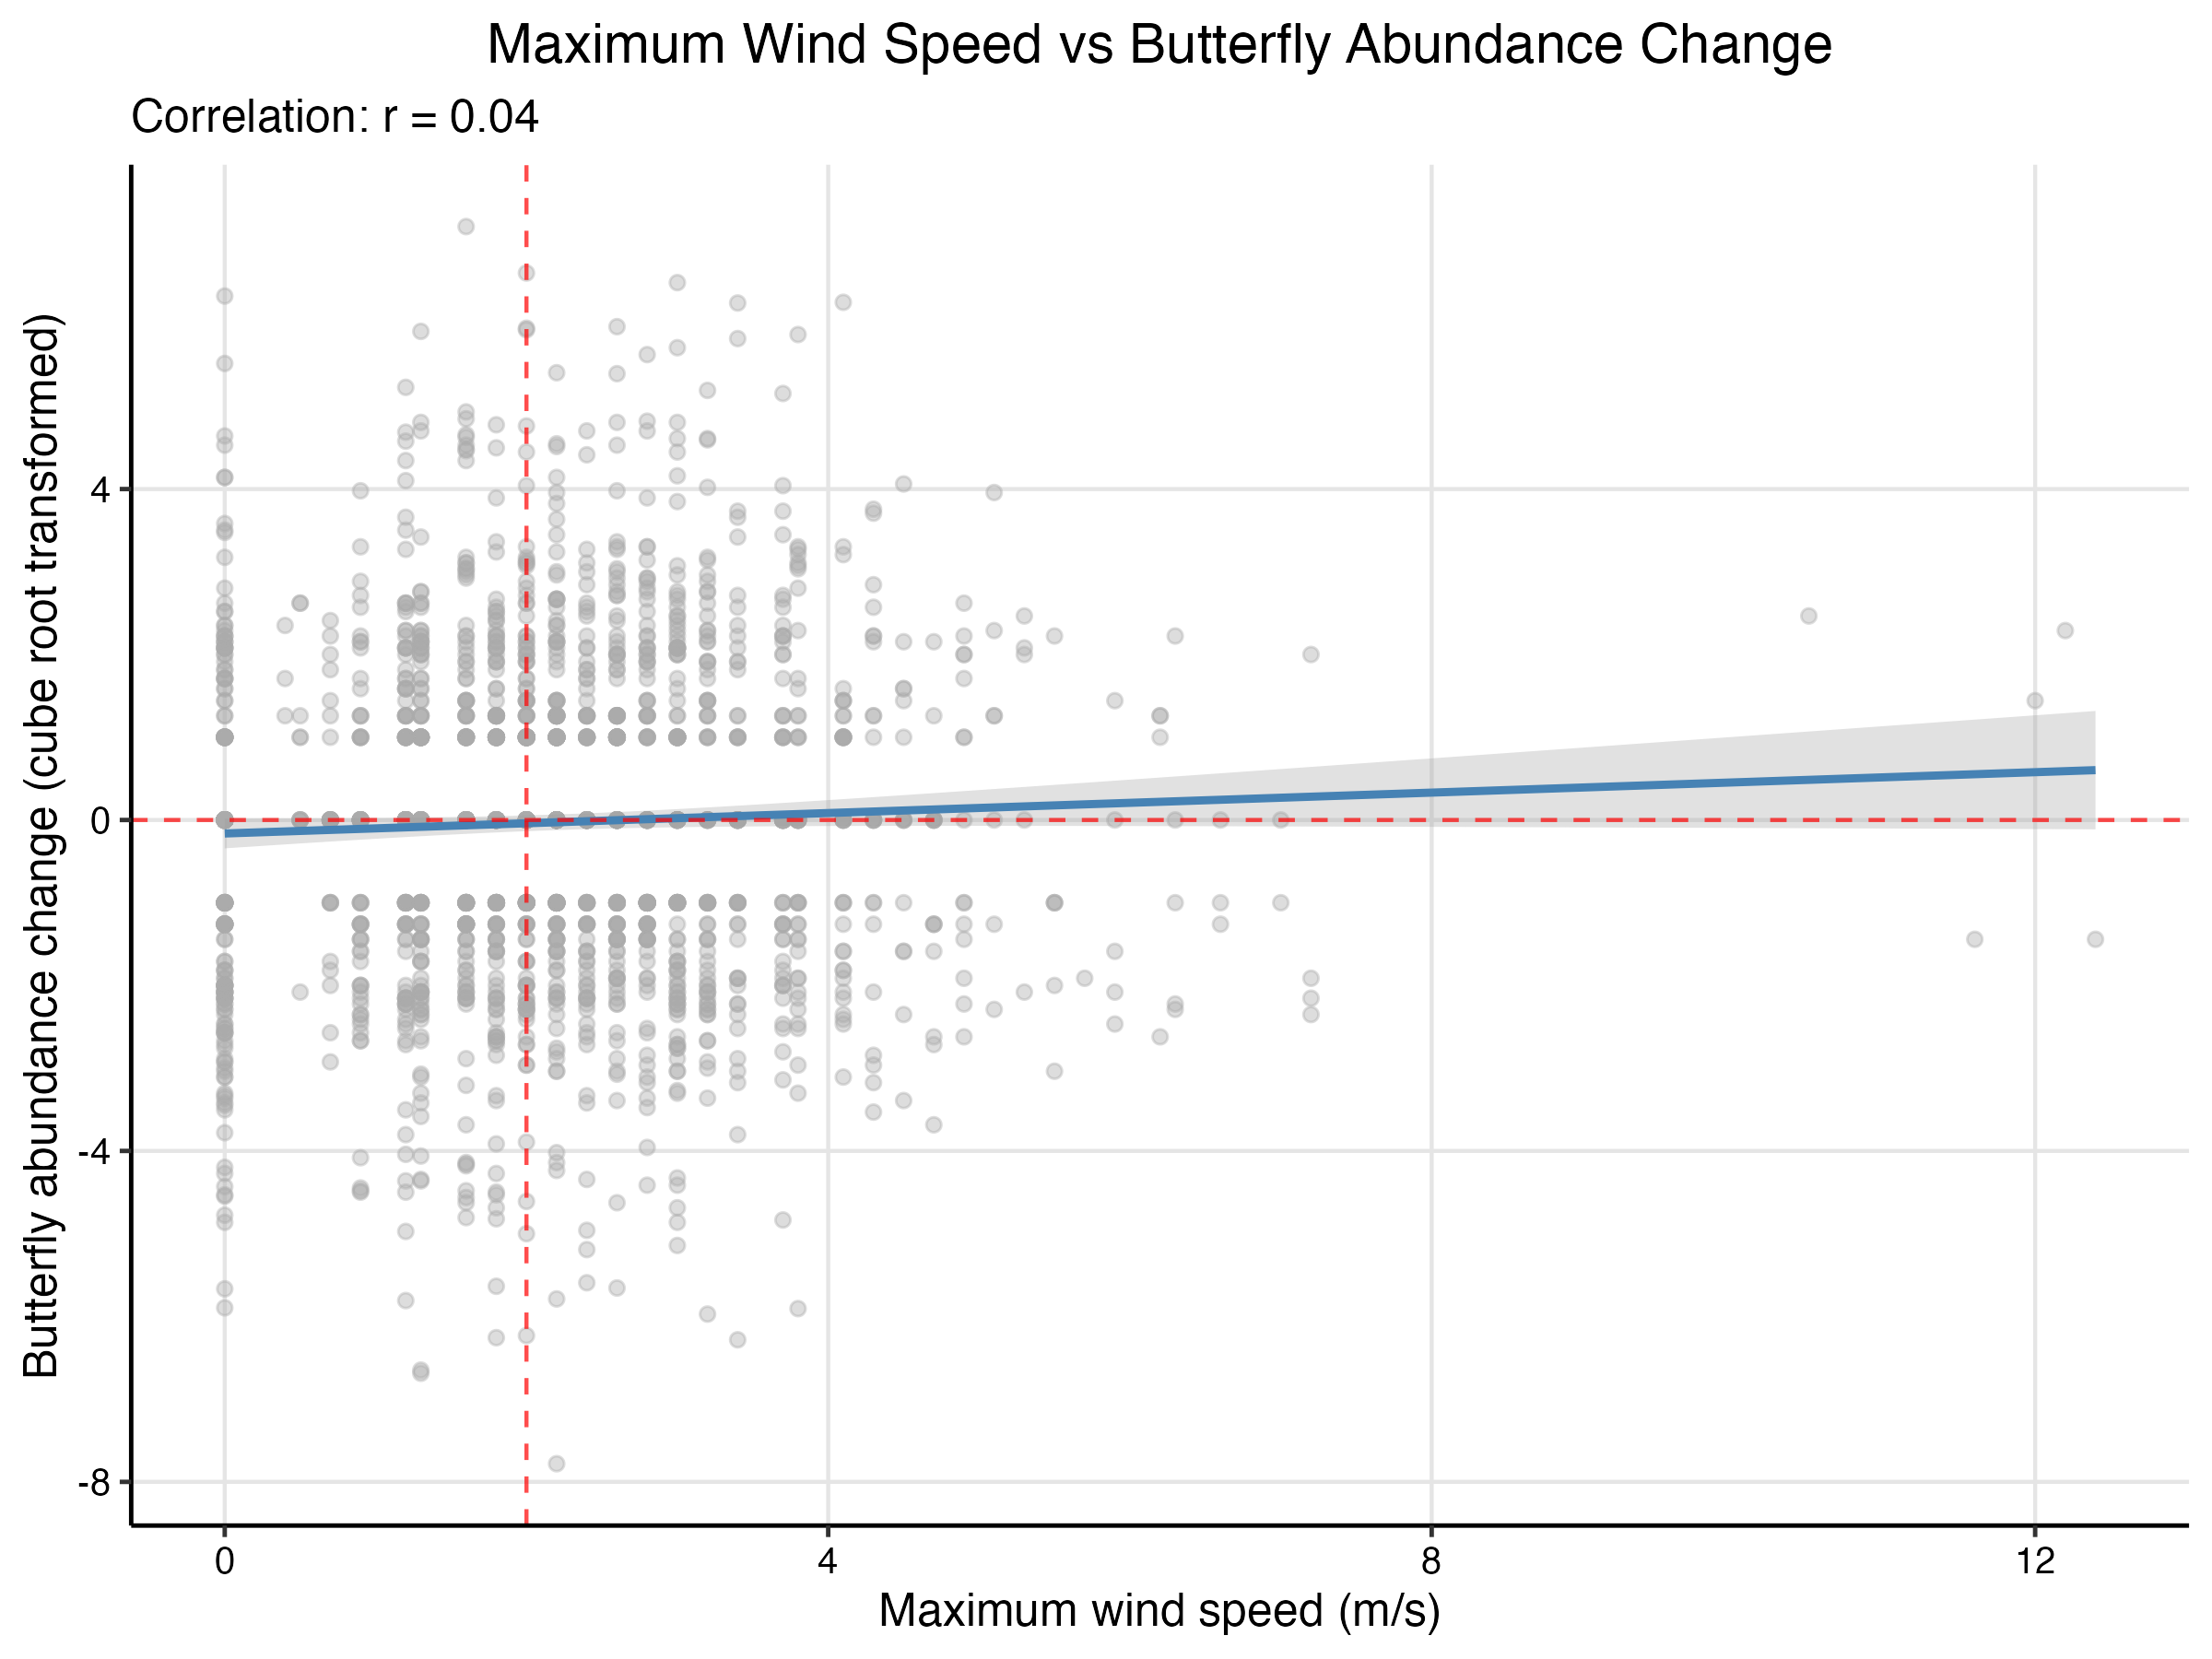
\includegraphics[width=0.8\textwidth]{figures/results/wind_hypothesis_scatter.png}
\caption{Relationship between maximum wind speed (m/s) and monarch abundance change. The red dashed line shows the proposed 2 m/s disruptive wind threshold, while the flat trend line indicates no effect of wind on butterfly departures. Points represent 30-minute observation periods.}\label{fig:wind_scatter}
\end{figure}

\subsection{Statistical Power to Detect Wind Effects}

Post-hoc power analysis confirmed our study had adequate statistical power to detect biologically meaningful wind effects (Table~\ref{tab:power_analysis}). With 1,894 paired observations, we achieved 87.5\% power to detect moderate effect sizes (0.15 standard deviations) and 98.5\% power to detect larger effects (0.20 standard deviations). Power for small effects (0.10 standard deviations) was 56\%, while very small effects (0.05 standard deviations) yielded only 16.5\% power. These results indicate that our failure to detect wind effects is unlikely due to insufficient statistical power for effect sizes of biological relevance.

\begin{table}[htbp]
\centering
\caption[Statistical power to detect wind effects]{Estimated power to detect wind effects of varying magnitudes. Effect sizes are expressed in standard deviations of the response variable (cube root transformed change in butterfly abundance).}
\label{tab:power_analysis}
\begin{tabular}[t]{lrrl}
\toprule
  & Effect Size (SD units) & Power (Proportion) & Power (\%)\\
\midrule
0.05 & 0.05 & 0.165 & 16.5\%\\
0.1 & 0.10 & 0.560 & 56\%\\
0.15 & 0.15 & 0.875 & 87.5\%\\
0.2 & 0.20 & 0.985 & 98.5\%\\
\bottomrule
\end{tabular}
\end{table}


\subsection{Model Diagnostics}

Model residuals showed distinct linear banding patterns consistent with the discrete counting method used to estimate butterfly abundance, while the Q-Q plot indicated approximately normal residual distribution with minor tail deviations (Figure~\ref{fig:diagnostics}).

\begin{figure}[htbp]
\centering
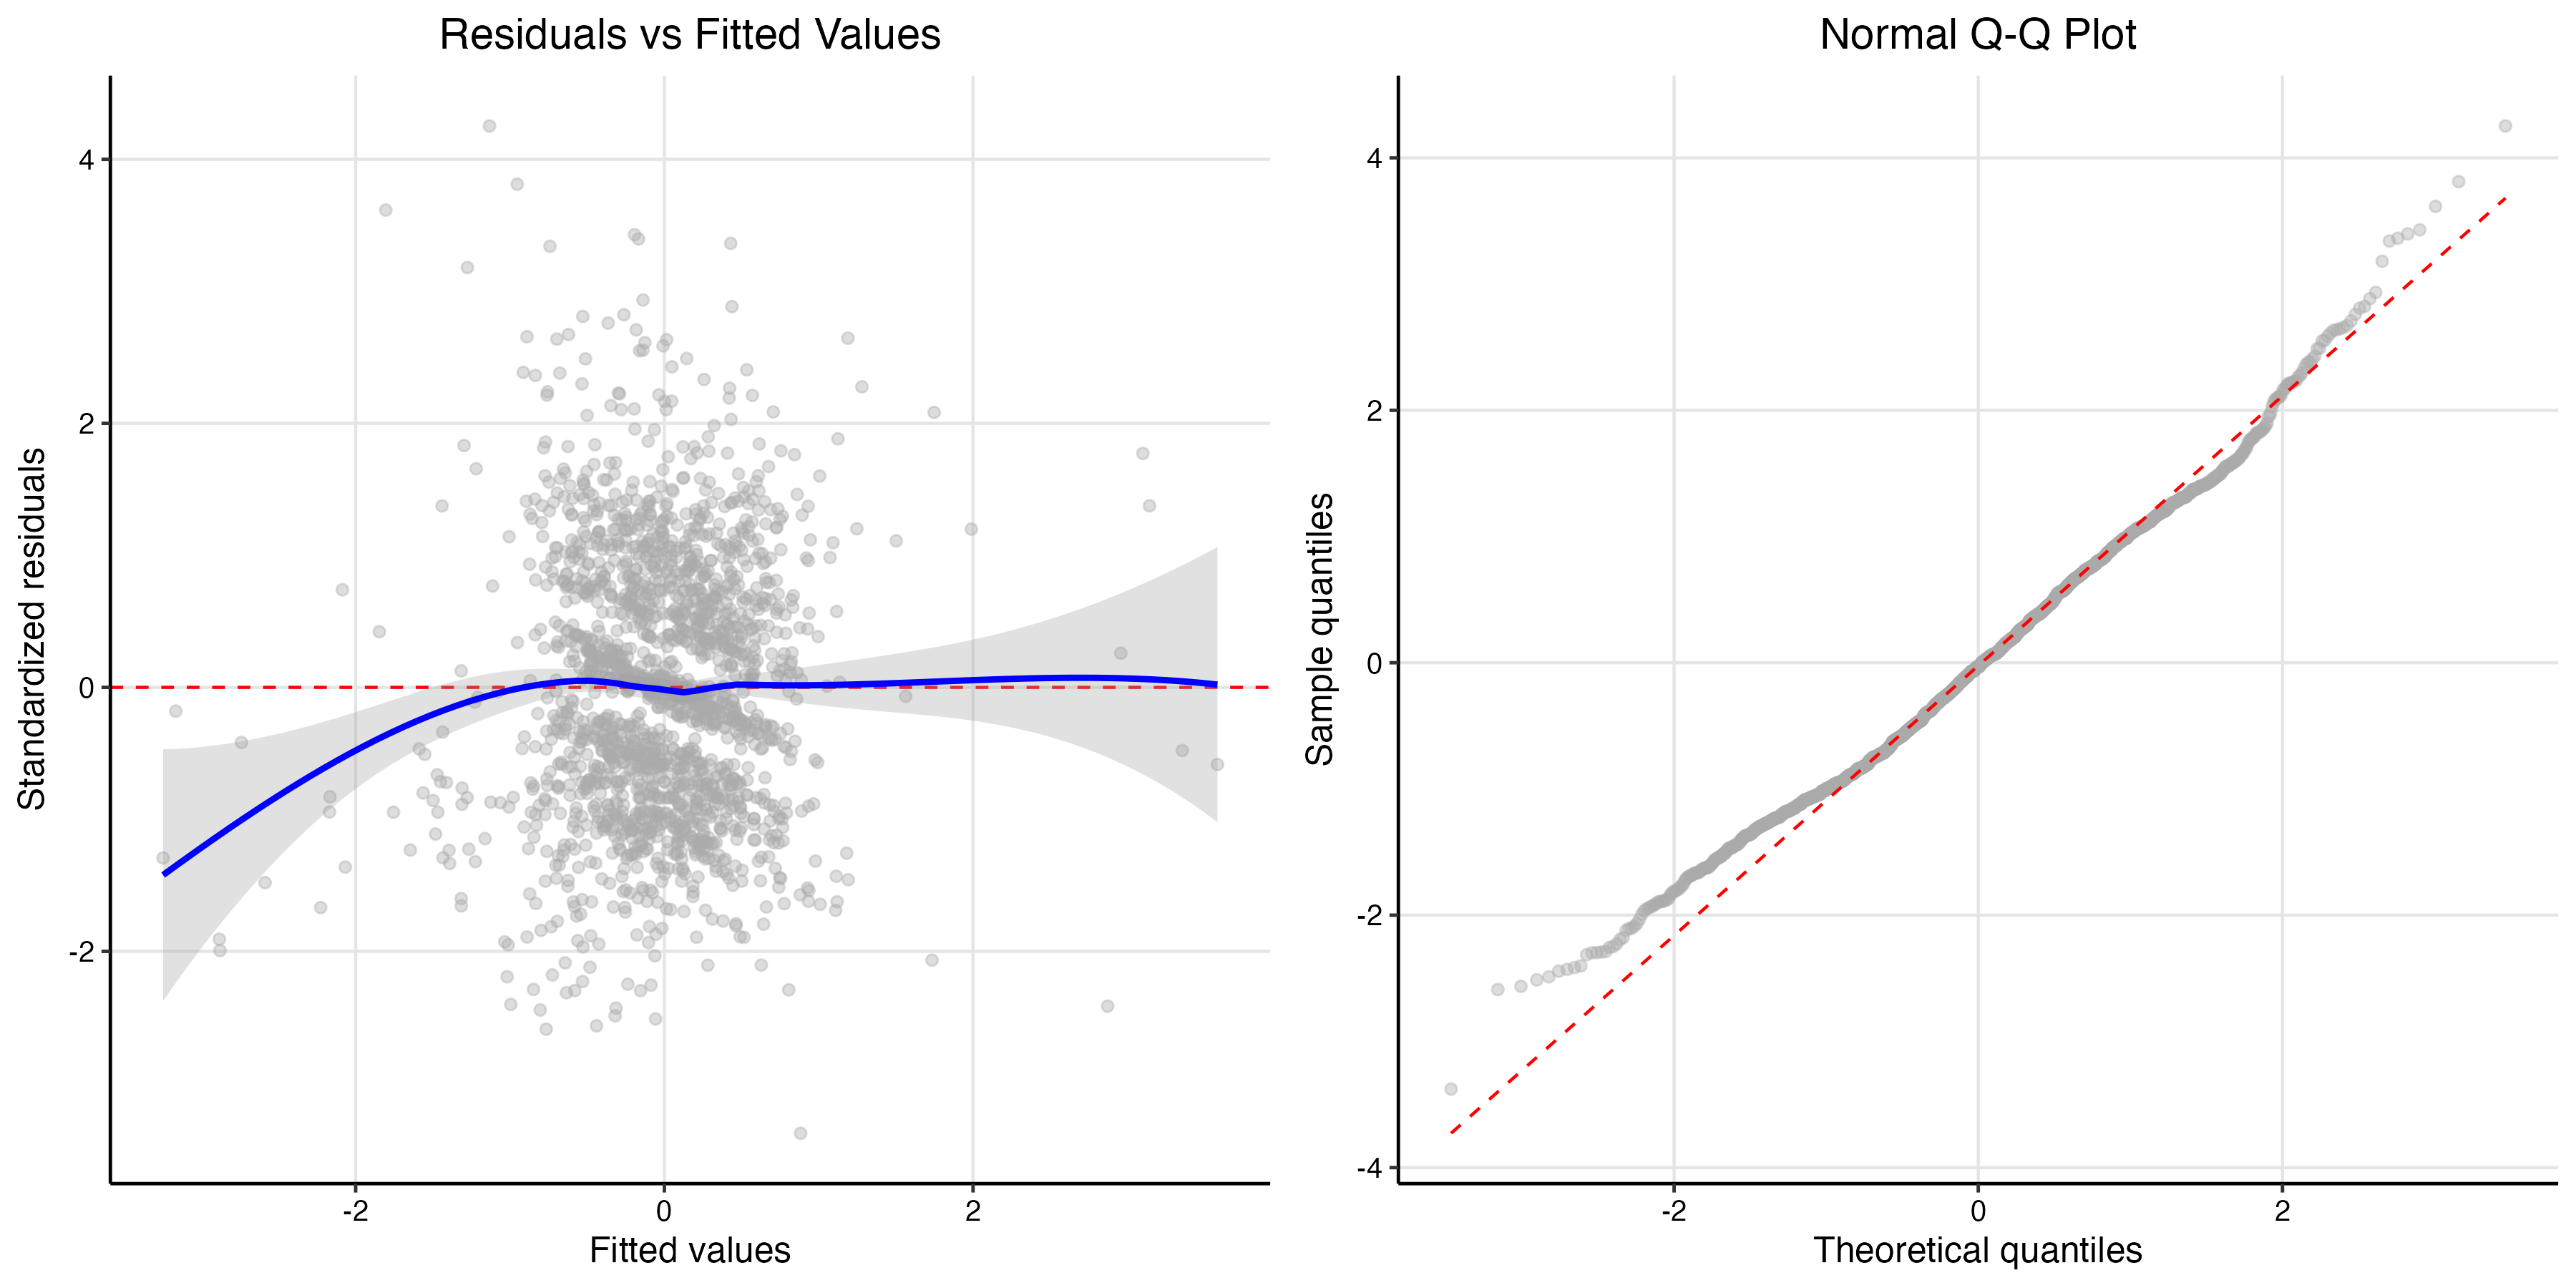
\includegraphics[width=\textwidth]{figures/results/combined_diagnostics.png}
\caption{Model diagnostics for M23. Left: Residuals versus fitted values showing banding that reflects the discrete counting method, with smoothed relationship shown in blue. Right: Normal Q-Q plot of model residuals showing reasonable normality with minor tail deviations.}\label{fig:diagnostics}
\end{figure}

% To update figures, rerun the quarto doc masters-analysis/analysis/monarch_gam_analysis.qmd (separate repo) and copy the thesis-exports folder to this one.